\section{Durchführung}
\label{sec:Durchführung}

\subsection{Aufbau}
\label{sec:Aufbau}

In Abbildung \ref{fig:aufbau} ist zunächst eine Aufnahme des Versuchsaufbau zu
sehen. Dabei befindet sich oben links eine Halbleiter-Laserdiode($\SI{405}{\nano\meter}$).
Das entsendete Licht fällt zunächst in einen optischen Isolator/Diode, welche
unerwünschte Rückreflexionen unterbindet und damit den Laser vor Störungen schützt.
Bei dem optischen Isolator wird der Faraday-Effekt genutzt, indem ein Faraday-Rotator,
welcher auf die Wellenlänge von $\SI{405}{\nano\meter}$ eingestellt ist,
zwischen zwei um $\SI{45}{\degree}$ zueinander verdrehte Polarisationsfilter
geschaltet wird. Licht aus dem Laser wird nun durch den Faraday-Rotator
um $\SI{45}{\degree}$ gedreht und passiert den dahinter geschalteten Polarisationsfilter.
Licht aus der anderen Richtung wird hingegen so gedreht, dass es den Filter nicht
mehr passieren kann.
Der dem optischen Isolator hintergeschaltende Gradientenfilter hat die Aufgabe,
die Laserleistung zu regulieren, damit darauffolgende Bauteile nicht übersteuert
werden. Dabei lässt sich die ausgehende Intensität über Ändernung des Polarwinkels
regulieren. Dem Gradientenfilter folgen eine $\lambda$/2-Platte und ein
Glan-Taylor-Prisma, welche beide auf dem Effekt der Doppelbrechung basieren. Bei
der Doppelbrechung wird das Licht in einen außerordentlichen und einem ordentlichen
Strahlanteil zerlegt, wobei beide Anteile nun linear polarisiert sind und deren
Polarisation senkrecht zueinander steht. Der ordentliche Anteil folgt dem
Snelliusschen Brechungsgesetz, wohingegen der außerordentliche Anteil diesem
eben nicht folgt. Beide Strahlanteile haben damit unterschiedliche Brechzahlen.
Die $\lambda$/2-Platte nutzt den Unterschied in der Brechzahlen, um die Phase
zwischen den beiden Anteilen um $\lambda$/2 zu drehen.

\begin{figure}[hbtp]
	\centering
	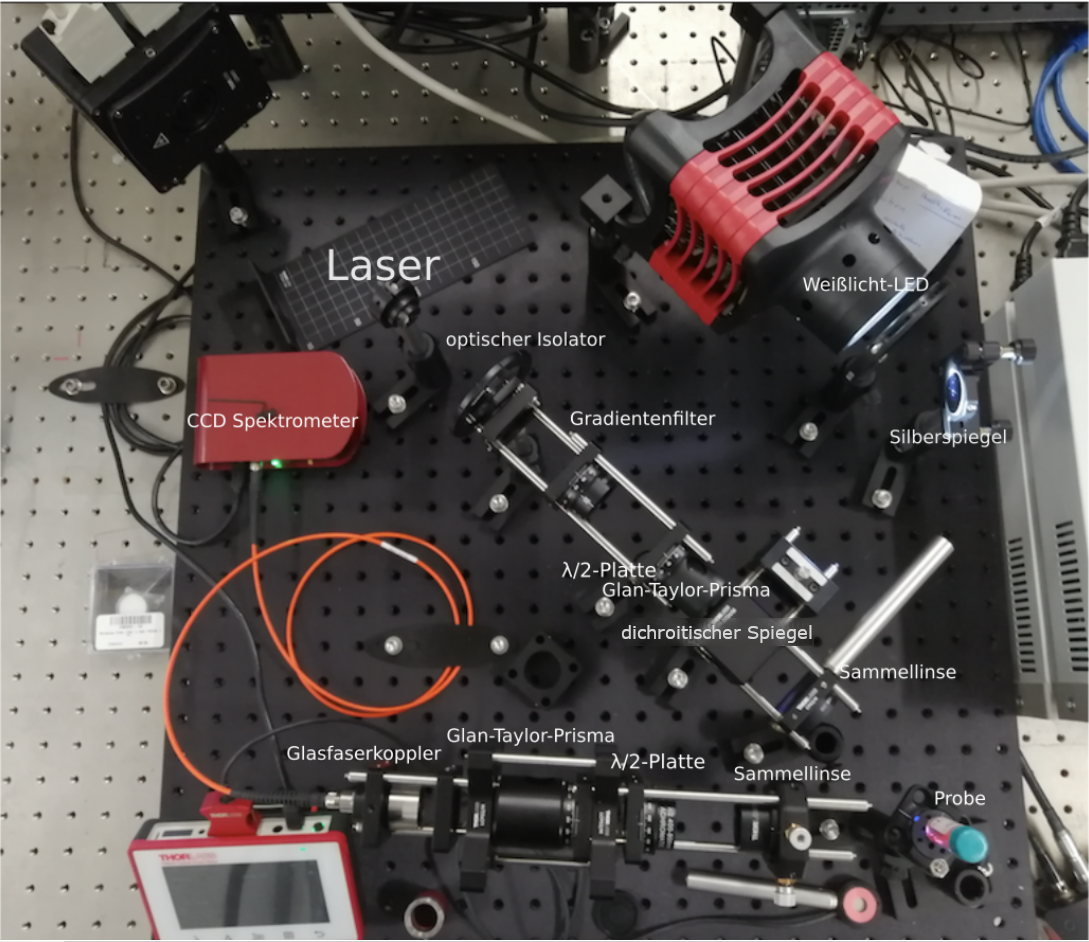
\includegraphics[width=\textwidth]{Abb/aufbau.png}
	\caption{Versuchsaufbau \cite{flex} zur Untersuchung der Photolumineszenz. Die
    hier dargestellte Weißlicht-LED-Quelle wird in diesem Versuch jeweils durch einen
    448, 518 und einem $\SI{636}{\nano\meter}$ Laser ausgetauscht. Ebenso wird in diesem
    Versuch auf die Sammellinse im Strahlengang verzichtet.}
	\label{fig:aufbau}
\end{figure}
\noindent
Ist die Polarisation nun richtig eingestellt, lässt sich der ordentliche
Strahlanteil rausfiltern und nur der außerordentliche Strahl kann das Primsa
passieren. Im letzten Schritt durchläuft das Licht durch den dichroischen Spiegel,
welcher nur Licht aber einer bestimmten Wellenlänge passieren lässt. Sinnvoll hintereinander
geschaltete Medien mit unterschiedlichen Brechzahlen lassen Wellenlängen unterhalb von
$\SI{435}{\nano\meter}$ destruktiv und Wellenlänge oberhalb konstruktiv interferieren.
Nun trifft das linear polarisiert Licht der Wellenlänge größer als $\SI{435}{\nano\meter}$
auf die Probe und es kommt zu den in der Theorie \ref{sec:Theorie} benannten Effekten,
welche mittels des Detektionpfades gemessen werden. Dazu wird die entsendete
Photolumineszenz zunächst mit einer Sammellinse (Brennweite $\SI{60}{\milli\meter}$)
gebündelt. Dann durchläuft das Licht wieder die Kombination aus $\lambda$/2-Platte
und dem Glan-Taylor-Prisma und wird schließlich durch einen Glasfaserkoppler in das
CCD Spektrometer geleitet.
Im weiteren Verlauf des Versuches wird ein weiterer Anregungspfad aufgebaut. Dabei
wird anstelle der in Abbildung \ref{fig:aufbau} dargestellten Weißlicht-LED-Quelle
jeweils ein Laser der Wellenlänge 448, 518 und $\SI{636}{\nano\meter}$
aufgestellt. Der Silberspiegelt erlaubt es dann, das Licht auf den dichroischen Spiegel
und damit auf die Probe zu leiten.\\

\subsection{Experiment}
\label{sec:Experiment}
Im ersten Versuchsteil wird die Nanokristallgröße der drei Proben anhand der Emissionsenergie
abgeschätz und ihre Polarisation untersucht. Dazu wird mittels des Gradientenfilters
und einem PM400-Laserleistungsmessgerät die Laserleistung auf etwa $\SI{1}{\milli\watt}$
eingestellt. Nachdem die Emissionsspektren aufgenommen sind, wird die Polarisations
im Detektionpfades auf $\SI{50}{\degree}$, $\SI{90}{\degree}$ und $\SI{180}{\degree}$
geändert.
Zuletzt wird für eine gewählte Probe die Abhängigkeit zwischen Anregungsleistung
(von 0,1 bis $\SI{20}{\milli\watt}$) und dem Verhalten des Emissionsspektrums
untersucht.\\
Im nächsten Versuchsteil wird der zweite Anregungspfad aufgebaut und
nacheinander die drei oben benannten Laser eingebaut. Für den jeweiligen Laser
wird dann erneuert das Emissionsspektrum für jede einzelne Probe aufgenommen.\\
Als letztes<s wird die Polarisation einer Weinprobe untersucht, indem Emissionsspektren
für vier Filtereinstellungen aus Kombinationen von $\SI{0}{\degree}$ und $\SI{90}{\degree}$
im Anregungs- und Detektionspfad vorgenommen werden. Dabei ist drauf zu achten,
dass eine Drehung an der  $\lambda$/2-Platte von $\SI{45}{\degree}$ einer Polarisation
von $\SI{90}{\degree}$ entspricht.
